\section{Durchführung}
\label{sec:Durchführung}

% Was wurde gemessen bzw. welche Größen wurden variiert?

\subsection{Bestimmung der Untergrundrate}
\label{ssec:d1}

Das erste Problem der Messung ist die Umgebungsradioaktivität, diese sollte so niedrig wie möglich gehalten werden.


\begin{figure}
    \centering
    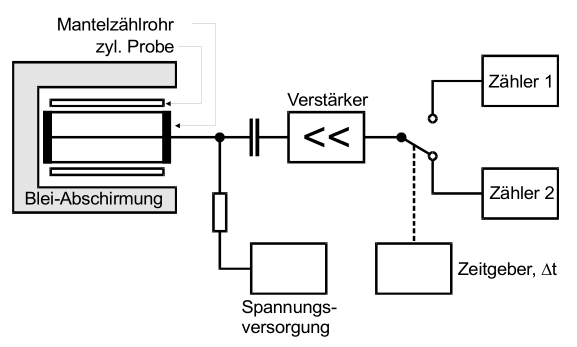
\includegraphics[width=\textwidth]{images/bild3.png}
    \caption{Schematischer Aufbau des Versuchs.}
    \label{fig:aufbau}
\end{figure}

\subsection{Bestimmung der Halbwertszeit von Vanadium}
\label{ssec:d2}

\subsection{Bestimmung der Halbwertszeit von Rhodium}
\label{ssec:d3}